%% LyX 2.3.6.2 created this file.  For more info, see http://www.lyx.org/.
%% Do not edit unless you really know what you are doing.
\documentclass[english]{beamer}
\usepackage{mathpazo}
\renewcommand{\sfdefault}{lmss}
\usepackage[T1]{fontenc}
\usepackage[latin9]{inputenc}
\usepackage{mathtools}
\usepackage{amsbsy}
\usepackage{amstext}
\usepackage{amssymb}
\usepackage{graphicx}

\makeatletter

%%%%%%%%%%%%%%%%%%%%%%%%%%%%%% LyX specific LaTeX commands.
%% Because html converters don't know tabularnewline
\providecommand{\tabularnewline}{\\}

%%%%%%%%%%%%%%%%%%%%%%%%%%%%%% Textclass specific LaTeX commands.
% this default might be overridden by plain title style
\newcommand\makebeamertitle{\frame{\maketitle}}%
% (ERT) argument for the TOC
\AtBeginDocument{%
  \let\origtableofcontents=\tableofcontents
  \def\tableofcontents{\@ifnextchar[{\origtableofcontents}{\gobbletableofcontents}}
  \def\gobbletableofcontents#1{\origtableofcontents}
}

%%%%%%%%%%%%%%%%%%%%%%%%%%%%%% User specified LaTeX commands.
\usetheme{Boadilla}
\usecolortheme{beaver}
%\usetheme{CambridgeUS}
% or ...
\usepackage{pgfpages}
%\setbeameroption{show notes}
\setbeameroption{show notes on second screen=right}

\setbeamercovered{transparent}
\setbeamertemplate{theorems}[numbered] 

\newcommand{\R}{\mathbb{R}}%
\newcommand{\T}{\mathcal{T}}%
\newcommand{\parens}[1]{\left(#1 \right)}%
\newcommand{\braces}[1]{\left\{#1 \right\}}%
\newcommand{\angles}[1]{\langle #1 \rangle}%
\newcommand\dd{\mathrm{d}}
\newcommand{\ddd}[1]{\frac{\dd}{\dd #1}}%
\newcommand{\dddd}[2]{\frac{\dd #1}{\dd #2}}%
\newcommand{\pd}[1]{\frac{\partial}{\partial #1}}%
\newcommand{\pdd}[2]{\frac{\partial #1}{\partial #2}}%
\newcommand{\evalat}[1]{\Big|_{#1}}%
\DeclareMathOperator*{\argmax}{argmax}%
\DeclareMathOperator*{\argmin}{argmin}%
\newcommand{\E}[1]{\text{E}\left[ #1 \right]}%

\@ifundefined{showcaptionsetup}{}{%
 \PassOptionsToPackage{caption=false}{subfig}}
\usepackage{subfig}
\makeatother

\usepackage{babel}
\begin{document}
\title{Non-linear protocols for optimal distributed consensus in networks
of dynamic agents}
\subtitle{D. Bauso and L. Giarre and R. Pesenti}
\author{Maksim Levental}

\makebeamertitle
\pgfdeclareimage[height=0.5cm]{institution-logo}{uchicago_logo.jpeg}

%\logo{\pgfuseimage{institution-logo}}


%\AtBeginSubsection[]{
%  \frame<beamer>{ 
%    %\frametitle{Outline}   
%    %\tableofcontents[currentsection,currentsubsection] 
%  }
%}
\AtBeginSection[]{
  \begin{frame}
  \vfill
  \centering
  \begin{beamercolorbox}[sep=8pt,center,shadow=true,rounded=true]{title}
    \usebeamerfont{title}\insertsectionhead\par%
  \end{beamercolorbox}
  \vfill
  \end{frame}
}
\AtBeginSubsection[]{
  \begin{frame}
  \vfill
  \centering
  \begin{beamercolorbox}[sep=8pt,center,shadow=true,rounded=true]{title}
    \usebeamerfont{title}\insertsubsectionhead\par%
  \end{beamercolorbox}
  \vfill
  \end{frame}
}

%\beamerdefaultoverlayspecification{<+->}
\begin{frame}{TLDR...}

\begin{figure}
\centering{}\includegraphics[width=0.75\linewidth]{tldr}
\end{figure}

\end{frame}

\begin{frame}{Outline}

\tableofcontents{}
\end{frame}

\section{Definitions}
\begin{frame}
\begin{definition}[Agents]
$\Gamma={1,\dots,n}$ is a set of \textit{agents/players/nodes/vertices}
and $G=(\Gamma,E)$ is a fixed (in time) undirected, connected, network
describing the connections between vertices $i\in\Gamma$, where $E\subset\Gamma\times\Gamma$
is the edge set. 

\end{definition}

\begin{definition}[Neighborhood]
A \textit{neighborhood} of a vertex $i$ is the set of all vertices
$j$ for which there is a single edge connecting $i,j$, that is to
say $N_{i}:=\left\{ j\mid(i,j)\in E\right\} $.
\end{definition}

\end{frame}
%
\begin{frame}
\begin{figure}
\begin{centering}
\includegraphics[width=0.5\linewidth]{neighbors1}\quad{}\includegraphics[width=0.33\linewidth]{neighbors2}\caption{Neighborhoods}
\par\end{centering}
\end{figure}
\end{frame}
%
\begin{frame}
\begin{definition}[Control policy]
Let $x_{i}(t)$ be the state of the agent $i$ at time $t$, then
$x_{i}$ evolves according to a \textit{distributed} and \textit{stationary}
control policy $u_{i}$, if $\dot{x}_{i}=u_{i}(x_{i},\mathbf{x}_{N_{i}})$,
where $\mathbf{x}_{N_{i}}$ are the states of $x_{i}$'s neighbors.
\end{definition}

\begin{definition}[Protocol]
The \textit{protocol} of the network is the collection of controls
$\mathbf{u}\left(\mathbf{x}\right):=\left(u_{i}\left(x_{i},\mathbf{x}_{N_{i}}\right)\right)$
for all $i\in\Gamma$.
\end{definition}

\end{frame}
%
\begin{frame}
\begin{definition}[Agreement function]
The \textit{agreement function} $\chi:\R^{n}\rightarrow\R$ is any
continuous, differentiable function which is permutation invariant,
i.e.
\[
\chi\left(\mathbf{x}\right)=\chi\left(x_{1},\dots,x_{n}\right)=\chi\left(x_{\sigma(1)},\dots,x_{\sigma(n)}\right)
\]
\end{definition}

\begin{definition}[Consensus]
To \textit{reach consensus} on \textit{consensus value} $\chi\left(\mathbf{x}\left(0\right)\right)$
means 
\[
\lim_{t\rightarrow\infty}\mathbf{x}\left(t\right)=\chi\left(\mathbf{x}\left(0\right)\right)\mathbf{1}
\]
 where $\mathbf{1}:=\left(1,1,\dots,1\right)$.
\end{definition}

\end{frame}

\section{The consensus problem}
\begin{frame}
\begin{definition}[Consensus problem]
Given a network $G$ of agents and agreement function $\chi$, the
\textit{consensus problem} is to design a protocol $\mathbf{u}$ such
that consensus is reached for any consensus value $\chi\left(\mathbf{x}\left(0\right)\right)$.
\end{definition}

\begin{definition}[Consensus protocol]
A protocol is a \textit{consensus protocol} if it is the solution
to a consensus problem. 
\end{definition}

\end{frame}

\subsection{Time-invariance of $\chi$}
\begin{frame}
\begin{lemma}[Time invariancy]
Let $\mathbf{u}$ be a stationary consensus protocol. Then $\chi(\mathbf{x}(t))$
is stationary, i.e. $\chi(\mathbf{x}(t))=\chi(\mathbf{x}(0))$ for
all $t>0$.
\end{lemma}

\begin{proof}
By assumption $\mathbf{x}\left(t\right)\rightarrow\chi\left(\mathbf{x}\left(0\right)\right)\mathbf{1}$.
Stationary $\mathbf{u}$ $\implies$ if $\mathbf{x}\left(t\right)$
is a solution, then $\mathbf{y}_{s}\left(t\right):=\mathbf{x}\left(t+s\right)$,
with $\mathbf{y}_{s}\left(0\right):=\mathbf{x}\left(s\right)$, is
also a solution. For such $\mathbf{y}_{s}$ we also have $\mathbf{y}_{s}\left(t\right)\rightarrow\chi\left(\mathbf{y}_{s}\left(0\right)\right)\mathbf{1}$,
i.e.
\[
\lim_{t\rightarrow\infty}\mathbf{y}_{s}\left(t\right)=\chi\left(\mathbf{y}_{s}\left(0\right)\mathbf{1}\right)=\chi\left(\mathbf{x}\left(s\right)\mathbf{1}\right)
\]
But since both $\mathbf{y}_{s},\mathbf{x}$ converge to the same limit
we must have $\chi\left(\mathbf{x}\left(s\right)\right)=\chi\left(\mathbf{x}\left(0\right)\right)$
for all $s$.
\end{proof}

\end{frame}
%
\begin{frame}

Note
\[
\dddd{\chi(\mathbf{x}(t))}{t}=\sum_{i\in\Gamma}\pdd{\chi}{x_{i}}\dot{x}_{i}=\sum_{i\in\Gamma}\pdd{\chi}{x_{i}}u_{i}=0
\]
Thus, a consensus protocol must satisfy $\nabla\chi\cdot\mathbf{u}=0$. 
\begin{example}
For $\chi(\mathbf{x})=\min_{i\in\Gamma}\left(x_{i}\right)$, a suitable
$\mathbf{u}$ is
\[
u_{i}=h\left(x_{i},\min_{j\in N_{i}}x_{j}\right)
\]
where $h(x,y)=0$ when $x=y$. 
\end{example}

\end{frame}
%
\begin{frame}

Henceforth, we assume further structure for the agreement function:

\begin{equation}
\chi(\mathbf{x})\coloneqq f\left(\sum_{i\in\Gamma}g(x_{i})\right)\label{eq:agreementfunctionform}
\end{equation}
with $f,g:\R\rightarrow\R$ and $g'\neq0$. 
\begin{fact}
Means of order $p$satisfy the assumptions

\begin{table}
\begin{centering}
\begin{tabular}{cccc}
\hline 
\noalign{\vskip1bp}
Mean & $\chi(\mathbf{x})$ & $f\text{\ensuremath{\left(y\right)}}$ & $g\text{\ensuremath{\left(z\right)}}$\tabularnewline[1bp]
\hline 
\noalign{\vskip1bp}
Arithmetic & $\frac{1}{\left|\Gamma\right|}\sum_{i\in\Gamma}x_{i}$ & $\frac{y}{\left|\Gamma\right|}$ & $z$\tabularnewline[1bp]
\noalign{\vskip1bp}
Geometric & $\left(\prod_{i\in\Gamma}x_{i}\right)^{1/\left|\Gamma\right|}$ & $e^{y/\left|\Gamma\right|}$ & $\log\left(z\right)$\tabularnewline[1bp]
\noalign{\vskip1bp}
Harmonic & $\frac{\left|\Gamma\right|}{\sum_{i\in\Gamma}x_{i}^{-1}}$ & $\frac{\left|\Gamma\right|}{y}$ & $\frac{1}{z}$\tabularnewline[1bp]
\noalign{\vskip1bp}
$p-$mean & $\left(\frac{1}{\left|\Gamma\right|}\sum_{i\in\Gamma}x_{i}^{p}\right)^{1/p}$ & $\left(\frac{y}{\left|\Gamma\right|}\right)^{1/p}$ & $z^{p}$\tabularnewline[1bp]
\end{tabular}
\par\end{centering}
\end{table}
\end{fact}

\end{frame}
%
\begin{frame}
\begin{theorem}[Protocol design rule]
The following protocol

\begin{equation}
u_{i}(x_{i},\mathbf{x}_{N_{i}}):=\frac{1}{g'}\sum_{j\in N_{i}}\phi(x_{j},x_{i})\label{eq:protocol}
\end{equation}
with $g'\neq0$, induces time-invariance in $\chi$ if $\phi$ is
antisymmetric, i.e. 

\[
\phi(x_{j},x_{i})=-\phi(x_{i},x_{j})
\]
\end{theorem}

\end{frame}
%
\begin{frame}
\begin{proof}
$\chi$ is time-invariant iff

\[
\dddd{}{t}\sum_{i\in\Gamma}g(x_{i})=\sum_{i\in\Gamma}\dddd{g(x_{i}(t))}{t}=\sum_{i\in\Gamma}\dddd{g(x_{i})}{x_{i}}\dot{x}_{i}=\sum_{i\in\Gamma}g'u_{i}=0
\]
Finally, since $\phi$ is antisymmetric and the graph defining the
network is undirected, we have that 

\[
\sum_{i\in\Gamma}g'u_{i}=\frac{1}{g'}\sum_{i\in\Gamma}g'\sum_{j\in N_{i}}\phi(x_{j},x_{i})=0
\]
\end{proof}

\end{frame}
%
\begin{frame}
\begin{example}[to be proved]
Consider $\phi(x_{j},x_{i}):=\alpha\cdot(x_{j}-x_{i})$. Then the
$p-$mean is time invariant under protocol
\[
u_{i}(x_{i},\mathbf{x}_{N_{i}}):=\frac{x_{i}^{1-p}}{p}\sum_{j\in N_{i}}\phi(x_{j},x_{i})=\alpha\cdot\frac{x_{i}^{1-p}}{p}\sum_{j\in N_{i}}(x_{j}-x_{i})
\]
\end{example}

\end{frame}
%

\subsection{Convergence of $\chi$}
\begin{frame}
\begin{itemize}
\item Owing to time-invariance of $\chi$, if the system converges, it will
converge to $\chi(\mathbf{x}(0))\mathbf{1}$. 
\item We prove convergence if
\[
\phi(x_{j},x_{i}):=\alpha\phi(\theta(x_{j})-\theta(x_{i}))
\]
with $\alpha>0$ and $\phi$ is continuous, $\theta:\R\rightarrow\R$
is differentiable with $\theta'$ locally Lipschitz and strictly positive. 
\item Thus, the protocol ($\ref{eq:protocol}$) becomes
\begin{equation}
u_{i}(x_{i},\mathbf{x}_{N_{i}}):=\frac{\alpha}{g'}\sum_{j\in N_{i}}\phi\left(\theta(x_{j})-\theta(x_{i})\right)\label{eqn:protocol2}
\end{equation}
with $g$ is strictly increasing.
\end{itemize}
\end{frame}
%
\begin{frame}
\begin{lemma}
Let $G$ be a network and $\mathbf{u}$ be a protocol with components
defined by eqn. ($\ref{eqn:protocol2}$). Then all equilibria $\mathbf{x}^{*}$
of the network have the following properties: 
\begin{enumerate}
\item $\mathbf{x}^{*}=\lambda\mathbf{1}$ for some $\lambda$ 
\item if $\mathbf{x}\left(t\right)$ converges to the equilibrium $\lambda_{0}\mathbf{1}$,
then $\lambda_{0}=\chi\left(\mathbf{x}\left(0\right)\right)$, for
any initial state $\mathbf{x}(0)$
\end{enumerate}
\end{lemma}

\begin{proof}[Proof (sketch)]
\begin{description}
\item [{Sufficiency\ 1}] $\mathbf{x}=\lambda\mathbf{1}$, then $\phi\left(\theta(\lambda)-\theta(\lambda)\right)=0$
since $\phi$ is odd and continuous.
\item [{Necessity\ 1}] $\mathbf{x}^{*}\neq\lambda$, then there exists
$u_{i}<0$ (contradicts equilibrium).
\item [{Convergence}] if $\lambda\neq\chi\left(\mathbf{x}\left(0\right)\right)$
then $\chi$ is not time-invariant.
\end{description}
\end{proof}

\end{frame}
%
\begin{frame}
\begin{theorem}
Let $G$ be a network of agents that implement a distributed and stationary
protocol
\[
u_{i}(x_{i},\mathbf{x}_{N_{i}}):=\frac{\alpha}{g'}\sum_{j\in N_{i}}\phi\left(\theta(x_{j})-\theta(x_{i})\right)
\]
against agreement function of the form (\ref{eq:agreementfunctionform})
with $g'>0$. Then the agents asymptotically reach consensus on $\chi\left(\mathbf{x}\left(0\right)\right)$
for any initial state $\mathbf{x}(0)$.

\end{theorem}

\end{frame}
%
\begin{frame}
\begin{proof}[Proof (idea)]
Define 
\[
\ensuremath{\eta_{i}:=g(x_{i})-g\left(\chi\left(\mathbf{x}\left(0\right)\right)\right)}
\]
and note that, since $\boldsymbol{\eta}$ is strictly increasing (since
$g$ is ) and $\boldsymbol{\eta}=0$ iff $\mathbf{x}=\chi\left(\mathbf{x}\left(0\right)\right)$,
consensus corresponds to asymptotic stability of $\boldsymbol{\eta}$
around $0$. Introduce a candidate Lyapunov function
\[
V\left(\boldsymbol{\eta}\right):=\frac{1}{2}\sum_{i\in\Gamma}\eta_{i}^{^{2}}
\]
Then $V\left(\boldsymbol{\eta}\right)=0$ iff $\boldsymbol{\eta}=0$,
$V\left(\boldsymbol{\eta}\right)>0$ if $\boldsymbol{\eta}\neq0$,
and $\dot{V}\left(\boldsymbol{\eta}\right)<0$ if $\boldsymbol{\eta}\neq0$
proves stability. 
\end{proof}

\end{frame}
%
\begin{frame}

\begin{figure}
\centering{}\includegraphics[width=0.75\linewidth]{Geometric-meaning-of-the-Lyapunov-function}\caption{Lyapunov function}
\end{figure}

\end{frame}
%

\section{Mechanism design problem}
\begin{frame}
\begin{definition}[Individual objective function]
Define an \textit{individual objective function} for an agent $i$
\[
J_{i}(x_{i},\mathbf{x}_{N_{i}},u_{i}):=\lim_{T\rightarrow\infty}\int_{0}^{T}\left(F(x_{i},\mathbf{x}_{N_{i}})+\rho u_{i}^{2}\right)\dd t
\]
where $\rho>0$ and $F:\R\times\R^{n}\rightarrow\R$ is a non-negative
\textit{penalty function.} A protocol is \textit{optimal} if each
$u_{i}$ optimizes an agent's corresponding individual objective.
\end{definition}

\begin{definition}[Mechanism design problem]
Consider a network of agents. The \textit{mechanism design problem}
is, for any agreement function $\chi$, to determine a penalty $F$
such that there exists an optimal consensus protocol $\mathbf{u}$
with respect to $\chi(\mathbf{x}(0))$ for any initial state $x(0)$.
\end{definition}

\end{frame}
%
\begin{frame}

Note that the mechanism design problem is over an infinite \textit{planning
horizon} $T\rightarrow\infty$. We need to discretize:
\begin{definition}
Let a one-step\textit{ action/planning period }be $\delta=t_{k+1}-t_{k}$.
Further let $\hat{x}_{i}\left(\tau,t_{k}\right)$ , $\hat{\mathbf{x}}_{N_{i}}\left(\tau,t_{k}\right)$,
$\hat{u}_{i}\left(\tau,t_{k}\right)$ be agent and neighboring states
and agent controls, for $\tau\geq t_{k}$. 

\end{definition}

Hence, we keep neighboring agents' states constant over a single planning
period and ultimately let $\delta\rightarrow0$ to get an approximation
to the original problem.
\end{frame}
%
\begin{frame}
\begin{block}{Receding horizon problem}
Define the \textit{receding horizon objective function}
\[
\hat{J}_{i}(\hat{x}_{i},\hat{\mathbf{x}}_{N_{i}},\hat{u}_{i}):=\lim_{T\rightarrow\infty}\int_{t_{k}}^{T}\left(\hat{F}(\hat{x}_{i}\left(\tau,t_{k}\right),\hat{\mathbf{x}}_{N_{i}}\left(\tau,t_{k}\right))+\rho\hat{u}_{i}^{2}\right)\dd\tau
\]
Then for all agents $i\in\Gamma$ and discrete time steps $t_{k}$,
given initial states $x_{i}(t_{0}),\mathbf{x}_{N_{i}}(t_{0})$ find
\[
\hat{u}_{i}^{*}:=\argmin\hat{J}_{i}(\hat{x}_{i},\hat{\mathbf{x}}_{N_{i}},\hat{u}_{i})
\]

subject to
\[
\begin{aligned}\dot{\hat{x}}_{i}(\tau,t_{k}) & =\hat{u}_{i}(\tau,t_{k})\\
\dot{\hat{x}}_{j}(\tau,t_{k}) & =\hat{u}_{j}(\tau,t_{k})=0\quad\forall j\in N_{i}\\
\hat{x}_{i}(t_{k},t_{k}) & =x_{i}(t_{k})\\
\hat{x}_{j}(t_{k},t_{k}) & =x_{j}(t_{k})\quad\forall j\in N_{i}
\end{aligned}
\]
\end{block}
\end{frame}
%
\begin{frame}

Note that the assumption that all neighboring states are fixed during
an action step implies 
\[
\hat{J}_{i}(\hat{x}_{i},\hat{u}_{i}):=\lim_{T\rightarrow\infty}\int_{t_{k}}^{T}\left(\hat{F}(\hat{x}_{i}(\tau,t_{k}))+\rho\hat{u}_{i}^{2}(\tau,t_{k})\right)\dd\tau
\]

Thus, we use Pontryagin's minimum principle.
\end{frame}
%
\begin{frame}
\begin{definition}[Pontryagin's minimum principle]
Let \textit{Hamiltonian }be

\[
H(\hat{x}_{i},\hat{u}_{i},p_{i})=L(\hat{x}_{i},\hat{u}_{i})+p_{i}\hat{u}_{i}
\]
where the \textit{Lagrangian} $L:=F(\hat{x}_{i}+\rho\hat{u}_{i}^{2})$.
Then $H$ abides by the Pontryagin necessary conditions at the optimum
$(\hat{x}_{i}^{\*},\hat{u}_{i}^{\*},p_{i}^{\*})$:

$\begin{aligned}\pdd{H}{\hat{u}_{i}}=0\Rightarrow p_{i}=-2\rho\hat{u}_{i} & \quad\text{optimality}\\
\dot{p}_{i}=-\pdd{H}{x_{i}} & \quad\text{multiplier}\\
\dot{\hat{x}}_{i}=-\pdd{H}{p_{i}}\Rightarrow\dot{\hat{x}}_{i}=\hat{u}_{i} & \quad\text{costate equation}\\
\frac{\partial^{2}H}{\partial\hat{u}_{i}^{2}}\evalat{\hat{x}_{i}=\hat{x}_{i}^{*},\hat{u}_{i}=\hat{u}_{i}^{*},p_{i}=p_{i}^{*}}\geq0\Rightarrow\rho\geq0 & \quad\text{minimality equation}\\
H(\hat{x}_{i}^{*},\hat{u}_{i}^{*},p_{i}^{*})=0 & \quad\text{boundary}
\end{aligned}
$
\end{definition}

\end{frame}
%
\begin{frame}
\begin{theorem}
Consider the penalty function
\[
F(\hat{x}_{i}(\tau,t_{k})):=\rho\left(\frac{1}{g'}\sum_{j\in N_{i}}\theta(x_{j}(t_{k}))-\theta(\hat{x}_{i}(\tau,t_{k}))\right)^{2}
\]
where $g$ is increasing, $\theta$ is concave, and $(1/g')$ is convex.
Then 

\[
\hat{u}_{i}^{*}:=\frac{\alpha}{g'}\sum_{j\in N_{i}}\theta(x_{j}(t_{k}))-\theta(x_{i}(\tau))
\]
solves the mechanism design problem.
\end{theorem}

\begin{proof}[Proof (idea)]
Check each of the conditions of Pontryagin's minimum principle.
\end{proof}

\end{frame}
%
\begin{frame}
\begin{corollary}
Taking $\delta\rightarrow0$ we get that the penalty function

\[
F(x_{i},\mathbf{x}_{N_{i}}):=\rho\left(\frac{1}{g'}\sum_{j\in N_{i}}\theta(x_{j})-\theta(x_{i})\right)^{2}
\]
and the optimal control law
\[
u_{i}(x_{i},\mathbf{x}_{N_{i}}):=\frac{1}{g'}\sum_{j\in N_{i}}\theta(x_{j})-\theta(x_{i})
\]
\end{corollary}

\end{frame}
%

\section{Simulations}
\begin{frame}

\begin{figure}
\centering{}\includegraphics[width=0.75\linewidth]{arith}
\end{figure}
\[
{\scriptstyle F:=\left(\sum_{j\in N_{i}}(x_{j}-x_{i})\right)^{2}\Rightarrow u_{i}=\sum_{j\in N_{i}}\left(x_{j}\left(t\right)-x_{i}\left(t\right)\right)\Rightarrow\lim_{t\rightarrow\infty}\chi\left(\mathbf{x}\left(t\right)\right)\rightarrow\frac{1}{\left|\Gamma\right|}\sum_{i\in\Gamma}x_{i}\left(0\right)}
\]

\end{frame}
%
\begin{frame}

\begin{figure}
\centering{}\includegraphics[width=0.75\linewidth]{geom}
\end{figure}
\[
{\scriptstyle F:=\left(\sum_{j\in N_{i}}x_{i}(x_{j}-x_{i})\right)^{2}\Rightarrow u_{i}=x_{i}\sum_{j\in N_{i}}\left(x_{j}\left(t\right)-x_{i}\left(t\right)\right)\Rightarrow\lim_{t\rightarrow\infty}\chi\left(\mathbf{x}\left(t\right)\right)\rightarrow\left(\prod_{i\in\Gamma}x_{i}\left(0\right)\right)^{1/\left|\Gamma\right|}}
\]

\end{frame}
%
\begin{frame}

\begin{figure}
\centering{}\includegraphics[width=0.75\linewidth]{harm}
\end{figure}
\[
{\scriptstyle F:=\left(x_{i}^{2}\sum_{j\in N_{i}}(x_{j}-x_{i})\right)^{2}\Rightarrow u_{i}=-x_{i}^{2}\sum_{j\in N_{i}}\left(x_{j}\left(t\right)-x_{i}\left(t\right)\right)\Rightarrow\lim_{t\rightarrow\infty}\chi\left(\mathbf{x}\left(t\right)\right)\rightarrow\frac{\left|\Gamma\right|}{\sum_{i\in\Gamma}\left(x_{i}\left(0\right)\right)^{-1}}}
\]

\end{frame}
%
\begin{frame}

\begin{figure}
\centering{}\includegraphics[width=0.75\linewidth]{two}
\end{figure}
\[
{\scriptstyle F:=\frac{1}{2x_{i}}\left(\sum_{j\in N_{i}}(x_{j}-x_{i})\right)^{2}\Rightarrow u_{i}=\frac{1}{2x_{i}}\sum_{j\in N_{i}}\left(x_{j}\left(t\right)-x_{i}\left(t\right)\right)\Rightarrow\lim_{t\rightarrow\infty}\chi\left(\mathbf{x}\left(t\right)\right)\rightarrow\sqrt{\frac{1}{\left|\Gamma\right|}\sum_{i\in\Gamma}\left(x_{i}\left(0\right)\right)^{2}}}
\]

\end{frame}
%
\begin{frame}
In general

\begin{align*}
F\left(x_{i},\mathbf{x}_{N_{i}}\right) & :=\left(\frac{x_{i}^{1-p}}{p}\sum_{j\in N_{i}}(x_{j}-x_{i})\right)^{2}\Rightarrow\\
u_{i}(x_{i},\mathbf{x}_{N_{i}}) & :=\frac{x_{i}^{1-p}}{p}\sum_{j\in N_{i}}(x_{j}-x_{i})\Rightarrow\\
\lim_{t\rightarrow\infty}\chi\left(\mathbf{x}\left(t\right)\right) & \;\rightarrow\left(\frac{1}{\left|\Gamma\right|}\sum_{i\in\Gamma}\left(x_{i}\left(0\right)\right)^{p}\right)^{1/p}
\end{align*}

\end{frame}
%

\section{Bonus 1: Graph Laplacian}
\begin{frame}
\begin{definitions}
The \textit{adjacency matrix} of a graph $G=\left(\Gamma,E\right)$
is defined
\[
\Delta A_{ij}\left(G\right)\coloneqq\begin{cases}
1 & \left(i,j\right)\in E\\
1 & \left(j,i\right)\in E\\
0 & \text{otherwise}
\end{cases}
\]
The \textit{degree matrix} of a graph $G$ is defined
\[
\Delta_{ij}\left(G\right)\coloneqq\begin{cases}
\deg\left(v_{i}\right) & i=j\\
0 & i\neq j
\end{cases}
\]
The \textit{Laplacian} of the graph $G$ is defined
\[
L\left(G\right)\coloneqq\Delta\left(G\right)-A\left(G\right)
\]
\end{definitions}

\end{frame}
%
\begin{frame}
\begin{theorem}
Suppose that each node $v\in G$ of a connected graph $G$ receives
the information from its neighboring nodes after a fixed delay $\delta>0$
and applies a linear protocol. Then for 
\[
\delta=\delta^{*}\coloneqq\frac{\pi}{2\lambda_{n}}\quad\lambda_{n}=\lambda_{\max}\left(L\right)
\]
where $\lambda_{i}$ are eigenvalues of the Laplacian, the system
has a globally asymptotically stable oscillatory solution with frequency
$\omega=\lambda_{n}$.

\end{theorem}

\end{frame}
%
\begin{frame}

\begin{figure}
\begin{minipage}[c]{0.35\linewidth}%
\subfloat{\centering{}\includegraphics[width=1\linewidth]{oscill}}%
\end{minipage}\quad{}%
\begin{minipage}[c]{0.6\linewidth}%
\subfloat{\centering{}\includegraphics[width=1\linewidth]{oscill2}}%
\end{minipage}

\end{figure}

\end{frame}
%

\section{Bonus 2: Computational Power}
\begin{frame}
\begin{definition}
$\mathsf{PSPACE}$ is the set of all decision problems that can be
solved by a Turing machine using a polynomial amount of space.

\end{definition}

\begin{figure}
\begin{minipage}[c]{0.45\linewidth}%
\subfloat{\centering{}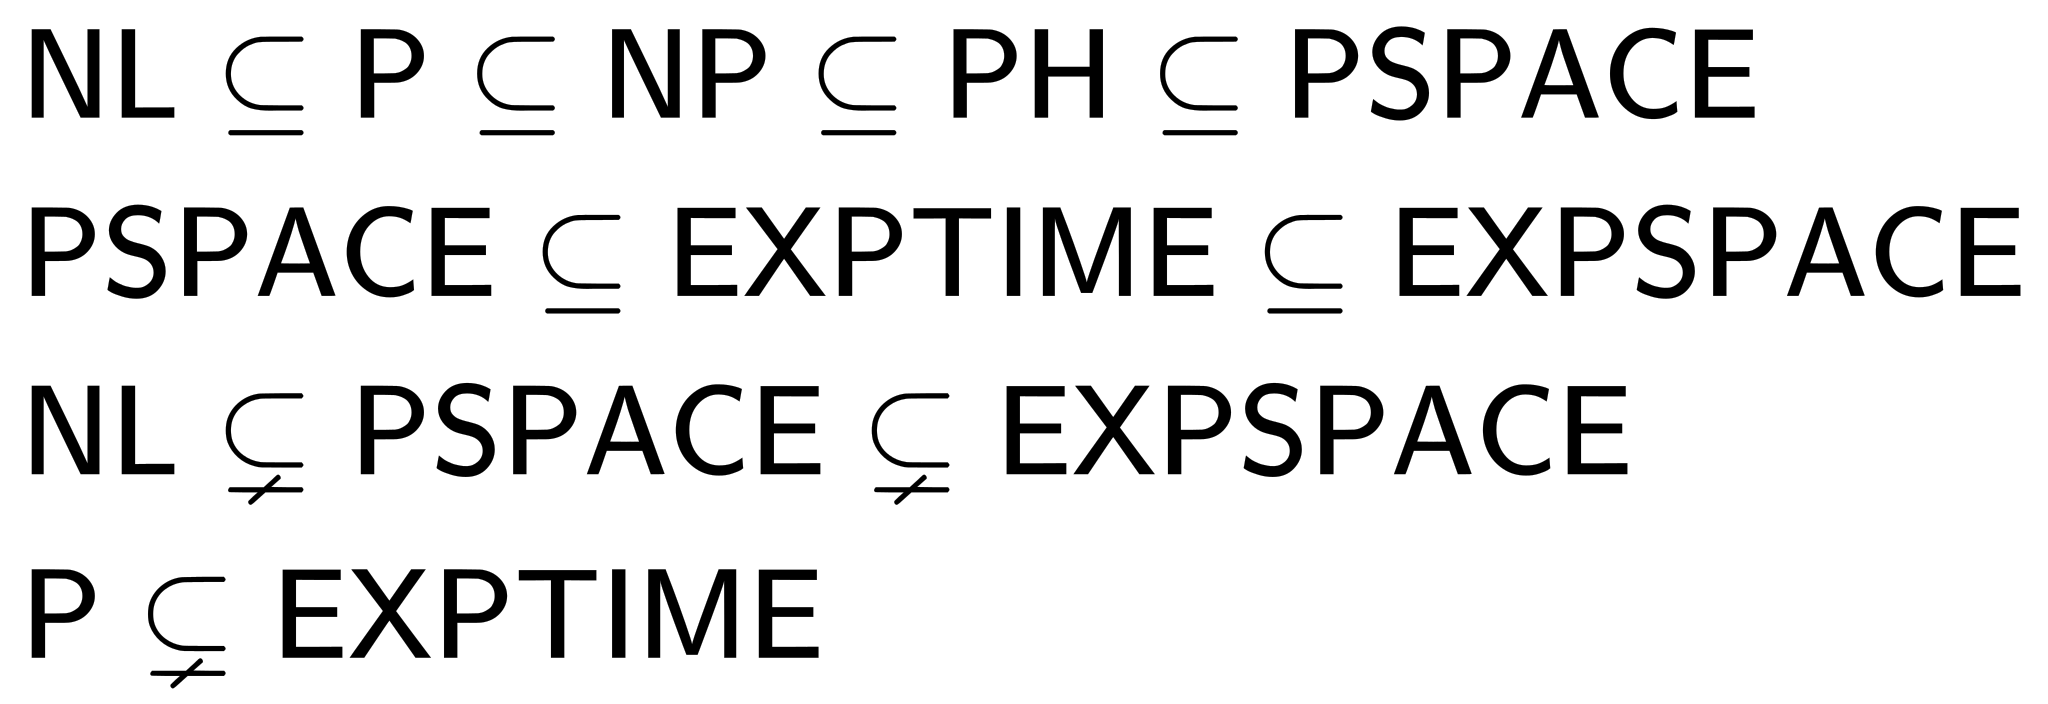
\includegraphics[width=1\linewidth]{inclusions}}%
\end{minipage}\quad{}%
\begin{minipage}[c]{0.45\linewidth}%
\subfloat{\centering{}\includegraphics[width=1\linewidth]{pspace}}%
\end{minipage}
\end{figure}

\end{frame}
%
\begin{frame}

``The computational power of networks of small resource-limited mobile
agents is explored. Two new models of computation based on pairwise
interactions of finite-state agents in populations of finite but unbounded
size are defined. With a fairness condition on interactions, the concept
of stable computation of a function or predicate is defined. Protocols
are given that stably compute any predicate in the class definable
by formulas of Presburger arithmetic, which includes Boolean combinations
of threshold-$k$, majority, and equivalence modulo $m$. All stably
computable predicates are shown to be in $\mathsf{NL}\coloneqq\mathsf{NSPACE}(\log n)$.
Assuming uniform random sampling of interacting pairs yields the model
of conjugating automata. Any counter machine with $O(1)$ counters
of capacity $O(n)$ can be simulated with high probability by a conjugating
automaton in a population of size $n$. All predicates computable
with high probability in this model are shown to be in $P$; they
can also be computed by a randomized logspace machine in exponential
time.''
\end{frame}
%
\begin{frame}

``Population protocols are a formal model of computation by identical,
anonymous mobile agents interacting in pairs. Their computational
power is rather limited: Angluin et al. have shown that they can only
compute the predicates over $\mathbf{\mathbb{N}}^{k}$ expressible
in Presburger arithmetic. For this reason, several extensions of the
model have been proposed, including the addition of devices called
cover-time services, absence detectors, and clocks. All these extensions
increase the expressive power to the class of predicates over $\mathbf{\mathbb{N}}^{k}$
lying in the complexity class \textbf{$\mathsf{NL}$} when the input
is given in unary. However, these devices are difficult to implement,
since they require that an agent atomically receives messages from
all other agents in a population of unknown size; moreover, the agent
must know that they have all been received. Inspired by the work of
the verification community on Emerson and Namjoshi\textquoteright s
broadcast protocols, we show that \textbf{$\mathsf{NL}$}-power is
also achieved by extending population protocols with reliable broadcasts,
a simpler, standard communication primitive.''

\end{frame}
%
\begin{frame}

``Broadcast consensus protocols (BCPs) are a model of computation,
in which anonymous, identical, finite-state agents compute by sending/receiving
global broadcasts. BCPs are known to compute all number predicates
in $\mathsf{NL}=\mathsf{NSPACE}(\log n)$ where $n$ is the number
of agents. They can be considered an extension of the well-established
model of population protocols. This paper investigates execution time
characteristics of BCPs. We show that every predicate computable by
population protocols is computable by a BCP with expected $O\left(n\log n\right)$
interactions, which is asymptotically optimal. We further show that
every log-space, randomized Turing machine can be simulated by a BCP
with $O\left(n\log n\cdot T\right)$ interactions in expectation,
where $T$ is the expected runtime of the Turing machine. This allows
us to characterise polynomial-time BCPs as computing exactly the number
predicates in $\mathsf{ZPL}$, i.e. predicates decidable by log-space
bounded randomised Turing machine with zero-error in expected polynomial
time where the input is encoded as unary.'' unary.''

\end{frame}
%
\begin{frame}[allowframebreaks]{Bibliography}

\bibliographystyle{plain}
\nocite{*}
\bibliography{biblio}
\end{frame}

\end{document}
